\begin{enumerate}[label=\thesection.\arabic*.,ref=\thesection.\theenumi]
\numberwithin{equation}{enumi}

\item For a unity feedback system given below refer, \ref{fig:ep18btech11016_block}, with
\begin{align}
    G\brak{s} &= \frac{K}{s\brak{s+5}\brak{s+11}}
    \label{eq:ep18btech11016_system}
\end{align}

\begin{figure}[h]
 \centering
    \resizebox{\columnwidth}{!}{\tikzstyle{block} = [draw, fill=white!20, rectangle, minimum height=3em, minimum width=4em]
\tikzstyle{sum} = [draw, fill=white!20, circle, node distance=1cm]
\tikzstyle{input} = [coordinate]
\tikzstyle{output} = [coordinate]
\tikzstyle{pinstyle} = [pin edge={to-,thin,black}]
\begin{tikzpicture}[auto, node distance=2cm,>=latex']
    
    \node [input, name=input] {};
    \node [sum, right of=input,node distance=2cm] (sum) {$\sum_{}^{}$};
    \node [block, right of=sum] (controller) {$C(s)$};
    \node [block, right of=controller,
            node distance=2.5cm] (system) {G(s)};
. 
    \draw [->] (controller) -- node[name=u] {} (system);
    \node [output, right of=system] (output) {};
    \coordinate [below of=u] (tmp);

    \draw [draw,->] (input) -- node  {$X(s) $} (sum);
    \draw [->] (sum) -- node {$ $} (controller);
    \draw [->] (system) -- node [name=y] {$Y(s) $}(output);
    \draw [->] (input) -- node{$ $} node[pos=0.93]{$+$} (sum);
    \draw [->] (y) |- (tmp) -| node[pos=0.99] {$-$} 
        node [near end] {$ $} (sum);
    
\end{tikzpicture}}
    \caption{}
    \label{fig:ep18btech11016_block}
\end{figure}

Find the value of the gain, K, of the uncompensated system operating at 30\% overshoot.\\

\solution\\ The damping ratio $\zeta$ is given by:

\begin{align}
    \zeta &= -\cfrac{\ln{\frac{\%OS}{100}}}{\sqrt{\pi^2 + \ln{\frac{\%OS}{100}}^2}}
    \label{eq:ep18btech11016_zeta}
\end{align}

Therefore, solving the above equation with \%OS = 30, we get,
\begin{align}
    \zeta &= 0.358
\end{align}

Further, we need to find the point on the root locus which crosses the 0.358 damping ratio line.\\
Let this point be $-\sigma_d + j\omega_d$, where $\sigma_d$ is the exponential damping frequency and $\omega_d$ is the damped frequency of oscillation.\\
And the relation between $\sigma_d$ and $\omega_d$ is given by,

\begin{align}
    \omega_d &= \sigma\tan\brak{\arccos{\zeta})}
\end{align}
where, 
\begin{align}
    \sigma_d &= \zeta\omega_n\\
    \omega_d &= \omega_n\sqrt{1-\zeta^2}
\end{align}
$\omega_n$ is the natural frequency.\\

Now, by solving the below equation and equating the real and imaginary parts to zero,

\begin{align}
    1 + G\brak{-\sigma_d + j\omega_d} &= 0
\end{align}
We get, 

\begin{align}
    \sigma_d &= 1.464\\
    \omega_d &= 3.818\\
    Gain, K &= 218.6
\end{align}

%-------------------------------------------------------------------------%

\item Evaluate the performance in terms of peak time and settling time as well as find $K_v$ of the uncompensated system.\\

\solution

The peak time, $T_p$ is given by,
\begin{align}
    T_p &= \frac{\pi}{\omega_d}
\end{align}

And, settling time is given by,
\begin{align}
    T_s &= \frac{4}{\sigma_d}
\end{align}

So, we get,
\begin{align}
    T_p &= 0.823\\
    T_s &= 2.732\\
    K_v &= \lim_{s \to 0} s G\brak{s}
\end{align}

\begin{align}
    \lim_{s \to 0} \brak{\frac{K}{\brak{s+5}\brak{s+11}}} &= \frac{218.6}{\brak{5}\brak{11}}\\
    \implies K_v &= 3.975
\end{align}

%-------------------------------------------------------------------------%

\item Design a lag-lead compensator to:
\begin{enumerate}
    \item Decrease the peak time by a factor of 2
    \item Decrease the percent overshoot by a factor of 2
    \item Improve the steady state error by a factor  of 30
\end{enumerate}

\solution\\
\textbf{Lead Design:}
Using the required specifications, we can calculate the damping ratio and the natural frequency,
Using eq. \ref{eq:ep18btech11016_zeta}, we get,
\begin{align}
    \zeta &= 0.517
\end{align}
And,
\begin{align}
    \omega_d = \frac{\pi}{T_p} = \omega_n\sqrt{1-\zeta^2} &= 7.634.
\end{align}
Hence, $\omega_n$ = 8.919.

Thus, the desired pole is located at,
\begin{align}
    -\zeta\omega_n + j\omega_n\sqrt{1-\zeta^2} &= -4.61 + j7.634
\end{align}

Let us now assume a lead compensator zero at -5. The summation of the system's original poles and lead compensator zero to the design point is -171.2$\degree$. Thus, the compensator pole must contribute 171.2$\degree$ - 180$\degree$ = -8.8$\degree$.

\begin{figure}[!ht]
 \centering
    \resizebox{\columnwidth}{!}{\tikzstyle{block} = [draw, fill=white!20, rectangle]
\tikzstyle{sum} = [draw, fill=white!20, circle, node distance=1cm]
\tikzstyle{input} = [coordinate]
\tikzstyle{output} = [coordinate]

\begin{tikzpicture}
    \draw[thick,->] (-3,0) -- (1,0);
    \draw[thick,->] (0,-0.5) -- (0,2);
    \draw (-0.8,0) -- (-0.8,0.9);
    \draw (0,0.9) -- (-0.8,0.9)
    \draw (-2.5,0) -- (-0.8,0.9)
    \draw[fill] (-2.5,0) circle [radius=0.04];
    
    \node[below] at (-2.5,0) {\scriptsize $-p_c$};
    \node[right] at (0,0.45) {\scriptsize j7.634};
    \node[below] at (-0.8,0) {\scriptsize -4.61};
    \node[below] at (1, 0) {\scriptsize $\sigma$};
    \node[above] at (0, 2) {\scriptsize $j\omega$};
    \node[above right] at (-2, 0) {\scriptsize $8.8\degree$};
    \node[above left] at (-1.5, 1.5) {\scriptsize s-plane}
    
\end{tikzpicture}   }
    \caption{}
    \label{fig:ep18btech11016_graph}
\end{figure}

Refer figure \ref{fig:ep18btech11016_graph} for clarification.

\begin{align}
    \tan\brak{8.8\degree} = \frac{7.634}{p_c - 4.61}
\end{align}
Hence, $p_c$ = 53.92.\\
Therefore, the compensated open-loop transfer function is,
\begin{align}
    \frac{K}{s\brak{s+11}\brak{s+53.92}}
\end{align}

Evaluating the gain for this function at the desired pole, we get $K = 4430$.\\

\textbf{Lag Design:}

The lead compensated $K_v$ = 7.469.\\
We need an improvement over the lead compensated system of,
\begin{align}
    \frac{\brak{30}\brak{3.975}}{7.469} &= \frac{119.25}{7.469}\\
    \implies &= 15.97
\end{align}

\begin{align}
K_v &= \lim_{s \to 0} s G\brak{s} 
\end{align}

Choose $p_c$ (compensator pole) = 0.001, we get $z_c$ (compensator zero) = 0.001597.
Thus, the compensator is given by, 
\begin{align}
    G_{lag}\brak{s} &= \frac{s+0.01597}{s+0.001}
\end{align}

So, the final compensated open loop transfer function is,
\begin{align}
    C\brak{s} G\brak{s} &= \frac{4430\brak{s+0.01597}}{s\brak{s+11}\brak{s+53.92}\brak{s+0.001}}
\end{align}

%-------------------------------------------------------------------------%

\item Plot the graph after adding a lag-lead compensator.

\solution\\
See Fig. \ref{fig:ep18btech11016_bode} generated by 
\begin{lstlisting}
codes/ep18btech11016/ep18btech11016.py
\end{lstlisting}

\begin{figure}[ht!]
    \centering
    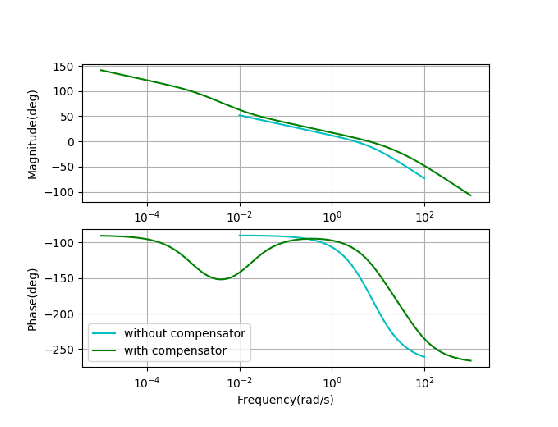
\includegraphics[width=\columnwidth]{./figs/ep18btech11016/ep18btech11016_fig3.eps}
    \caption{}
    \label{fig:ep18btech11016_bode}
\end{figure}

\end{enumerate}
